\documentclass[12pt]{article}

\usepackage{tikz}
\usetikzlibrary{positioning,arrows,calc}
 \def\nodedist{35pt}
\def\layerdist{80pt}
\def\pindist{20pt}


\begin{document}
	\begin{center}
		
		
		
		
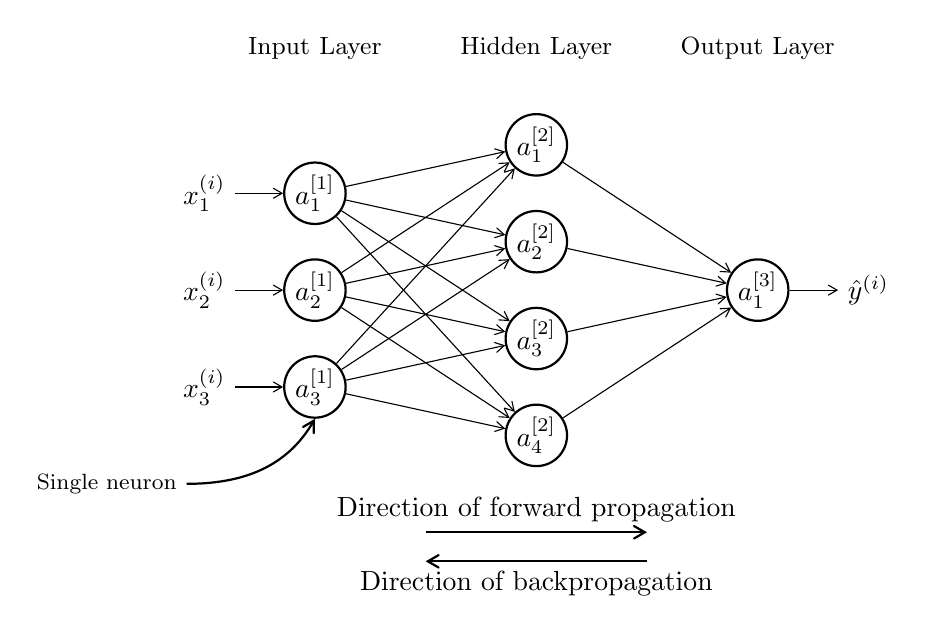
\begin{tikzpicture}[neuron/.style={circle,draw, thick,align=center, minimum size=2em,inner sep=1pt}, input/.style={->}]

\node[text width=2cm, align=center] at (0,.5*\nodedist) {\small Input Layer};

\node[text width=2cm, align=center] at (\layerdist,.5*\nodedist) {\small Hidden Layer};

\node[text width=2cm, align=center] at (2*\layerdist,.5*\nodedist) {\small Output Layer};

\foreach \y in {1,...,3} \node[] (in\y) at (-\layerdist*.5,-\y*\nodedist) {$x_\y^{(i)}$};  

\foreach \y in {1,...,3} \node[neuron]  (I\y) at (0,-\y*\nodedist) {$a_\y^{[1]}$};  

\foreach \in in {1,...,3} \draw[->, >=angle 60] (in\in) --  (I\in);

\foreach \y in {1,...,4} \node[neuron]  (H\y) at ($(\layerdist,-\y*\nodedist) +(0, .5*\nodedist)$) {$a_\y^{[2]}$};

\foreach \y in {1,...,1} \node[neuron] (O\y) at ($(I2) + (2*\layerdist, 0)$) {$a_\y^{[3]}$};

\node at ($(I2) + (2.5*\layerdist, 0)$) (y) {$\hat{y}^{(i)}$};


\foreach \dest in {1,...,4} \foreach \source in {1,...,3} \draw[->, >=angle 60] (I\source) -- (H\dest);

\foreach \dest in {1,...,1} \foreach \source in {1,...,4} \draw[->, >=angle 60] (H\source) -- (O\dest);

\draw[->, >=angle 60] (O1) -- (y);

\draw[->,  thick, >=angle 60] (.5*\layerdist,-4.5*\nodedist) -- node[above] {Direction of forward propagation} (1.5*\layerdist,-4.5*\nodedist);
\draw[->,  thick, >=angle 60]  (1.5*\layerdist,-4.8*\nodedist)-- node[below] {Direction of backpropagation} (.5*\layerdist,-4.8*\nodedist);
\node [anchor=west] (note) at (-1.3*\layerdist,-4*\nodedist) {\footnotesize Single neuron};
\draw [->,  thick, >=angle 60] (note) to[out=0, in=-120] (I3.south);
\end{tikzpicture}
		
		
		
	\end{center}


\end{document}